\documentclass[conference]{IEEEtran}
\IEEEoverridecommandlockouts
% The preceding line is only needed to identify funding in the first footnote. If that is unneeded, please comment it out.
\usepackage{cite}
\usepackage{amsmath,amssymb,amsfonts}
\usepackage{algorithmic}
\usepackage{graphicx}
\usepackage{textcomp}
\usepackage{xcolor}
\def\BibTeX{{\rm B\kern-.05em{\sc i\kern-.025em b}\kern-.08em
    T\kern-.1667em\lower.7ex\hbox{E}\kern-.125emX}}
\begin{document}

\title{Enhanced Quantitative Trading Strategies through Sentiment Analysis Using Large Language Models}

\author{\IEEEauthorblockN{1\textsuperscript{st} Wentao Ye}
\IEEEauthorblockA{\textit{SIGS} \\
\textit{Tsinghua University}\\
Shenzhen, China \\
yewt23@mails.tsinghua.edu.cn}
\and
\IEEEauthorblockN{2\textsuperscript{nd} Huaxuan Li}
\IEEEauthorblockA{\textit{SIGS} \\
\textit{Tsinghua University}\\
Shenzhen, China \\
lhx23@mails.tsinghua.edu.cn}
\and
\IEEEauthorblockN{3\textsuperscript{rd} Jiadong Li}
\IEEEauthorblockA{\textit{SIGS} \\
\textit{Tsinghua University}\\
Shenzhen, China \\
lijd23@mails.tsinghua.edu.cn}
}

\maketitle

\begin{abstract}
The stock market's significant price volatility necessitates sophisticated and adaptive trading strategies. Traditional quantitative trading strategies relying on historical market data face limitations. This project integrates sentiment analysis using large language models (LLMs) to enhance high frequency trading (HFT) strategies. By incorporating real-time sentiment analysis from news articles and social media, we aim to improve trading performance, decision-making, and overall profitability in high frequency trading.
\end{abstract}

\begin{IEEEkeywords}
High Frequency Trading, Sentiment Analysis, Large Language Models, Stock Market, Trading Strategies
\end{IEEEkeywords}

\section{\textbf{Introduction}}

\subsection{\textbf{Strategy Premise}}

\subsubsection{\textbf{Characteristics of the Stock Market}}
The stock market is characterized by its significant price volatility driven by factors such as market sentiment, speculative trading, and news events. This volatility creates opportunities for profit but also introduces risk, necessitating sophisticated trading strategies.

\subsubsection{\textbf{Limitations of Traditional Quantitative Trading Strategies}}
Traditional strategies rely on historical data and often neglect emotional and psychological factors. These strategies struggle to incorporate unstructured data from social media and news, presenting an opportunity for enhancement through sentiment analysis.

\section{\textbf{Method}}
\subsection{\textbf{LLM Fine-Tuning Methods Based on Sentiment Data}}

\begin{figure}[h]
    \centering
    \includegraphics[width=0.5\textwidth]{lora.png}
    \caption{The Low-rank Adaptation Method.}
    \label{fig:lora}
\end{figure}

In our project, we leverage LoRA (Low-Rank Adaptation) to fine-tune Llama 3, a state-of-the-art large language model, for sentiment analysis tasks. This approach enables the language model to accurately interpret and classify sentiments from textual data collected from news and social media. 

LoRA is designed to make the fine-tuning of large models more efficient. Traditional fine-tuning of models like Llama 3 can be computationally expensive and resource-intensive. LoRA addresses this by introducing low-rank parameter matrices into the model's architecture. These matrices significantly reduce the number of parameters that need to be updated during fine-tuning, making the process faster and less resource-demanding without compromising performance.

The fine-tuning process starts by initializing the pre-trained Llama 3 model. The pre-trained weights provide a solid foundation, having been trained on diverse and extensive datasets. LoRA layers are then integrated into Llama 3. These layers are low-rank matrices that capture task-specific adjustments, minimizing computational costs by only fine-tuning these layers. The training environment is configured, including setting hyperparameters such as learning rate, batch size, and number of epochs. Training and validation datasets are set up to ensure the model is trained on diverse sentiment-labeled texts.

During fine-tuning, the model learns to adjust its weights based on the sentiment data. The LoRA layers capture the nuances of sentiment classification, updating only a small portion of the model's parameters, ensuring the process is efficient and effective. After initial fine-tuning, the model's performance is evaluated using metrics like accuracy, precision, recall, and F1-score on a validation set. Based on the performance, we may iterate on the fine-tuning process, adjusting hyperparameters or incorporating more data to improve the model's accuracy.

The adoption of LoRA for fine-tuning Llama 3 offers several advantages. LoRA significantly reduces the computational resources required for fine-tuning large models. The fine-tuning process is faster due to the lower number of parameters being adjusted. Despite the reduced computational load, LoRA maintains high performance in task-specific adjustments. This approach allows for scalable fine-tuning, making it feasible to adapt Llama 3 for various specific tasks beyond sentiment analysis.

Once fine-tuned, Llama 3 is integrated into our sentiment analysis pipeline. The model processes real-time data from news and social media, classifying sentiments accurately and efficiently. The estimated sentiment value can therefore be used for downstream tasks. Utilizing LoRA for fine-tuning Llama 3 exemplifies a powerful and efficient approach to adapting LLMs for specific tasks such as sentiment analysis. This method not only enhances the model's capability to interpret sentiment but also ensures that the fine-tuning process is resource-efficient and scalable.

\subsection{\textbf{Quantitative Trading Framework}}

In quantitative investment, daily trading (such as portfolio management) and intraday trading (such as order execution) are typically analysed separately. However, to accurately evaluate the combined performance of these strategies, it is essential to integrate and backtest them together. This requires a robust framework capable of supporting multi-level joint backtesting.

Most existing quantitative trading frameworks do not account for multi-level joint trading, leading to inaccurate backtesting outcomes. Additionally, optimizing strategies at different levels is interdependent. For example, the best portfolio management strategy might change depending on the efficiency of order execution strategies. A portfolio with a higher turnover could be more advantageous if order execution is improved.

To achieve the best overall performance, it is necessary to consider how strategies at different levels interact. This quantitative trading framework not only enables precise joint backtesting but also ensures that the optimization of strategies at various levels is interconnected, thereby improving overall performance. By adopting this nested approach, we can comprehensively evaluate and optimize trading strategies, ensuring that enhancements in one area positively impact results in another. The input features used in our case include traditional quantitative factors and some newly introduced factors which will be discussed in the feature selection section.

The design of the framework is illustrated in Figure \ref{fig:framework}. Each level comprises a Trading Agent and an Execution Environment (Execution Env). The Trading Agent includes a data processing module (Information Extractor), a forecasting module (Forecast Model), and a decision generator (Decision Generator). The Forecast Model seeks to find alpha and assess risk. The trading algorithm uses the Decision Generator to optimize the investment portfolio based on the trading signals produced by the Forecast Model. These decisions are then sent to the Execution Env, which provides the execution results.

Our framework can customize the frequency of the trading algorithm, the decision content, and the execution environment to suit their needs (e.g., intraday trading, daily-frequency trading, weekly-frequency trading). Furthermore, the Execution Env can be nested with more granular trading algorithms and execution environments within it. For instance, daily-frequency orders can be split into finer-grained decisions for execution throughout the day.

The flexibility of this nested decision execution framework enables us to explore the effects of combining different levels of trading strategies and to overcome optimization barriers between various levels of trading algorithms. This comprehensive approach facilitates a thorough evaluation and optimization of trading strategies across different timeframes and execution granularities, enhancing overall trading performance.

\begin{figure}[h]
    \centering
    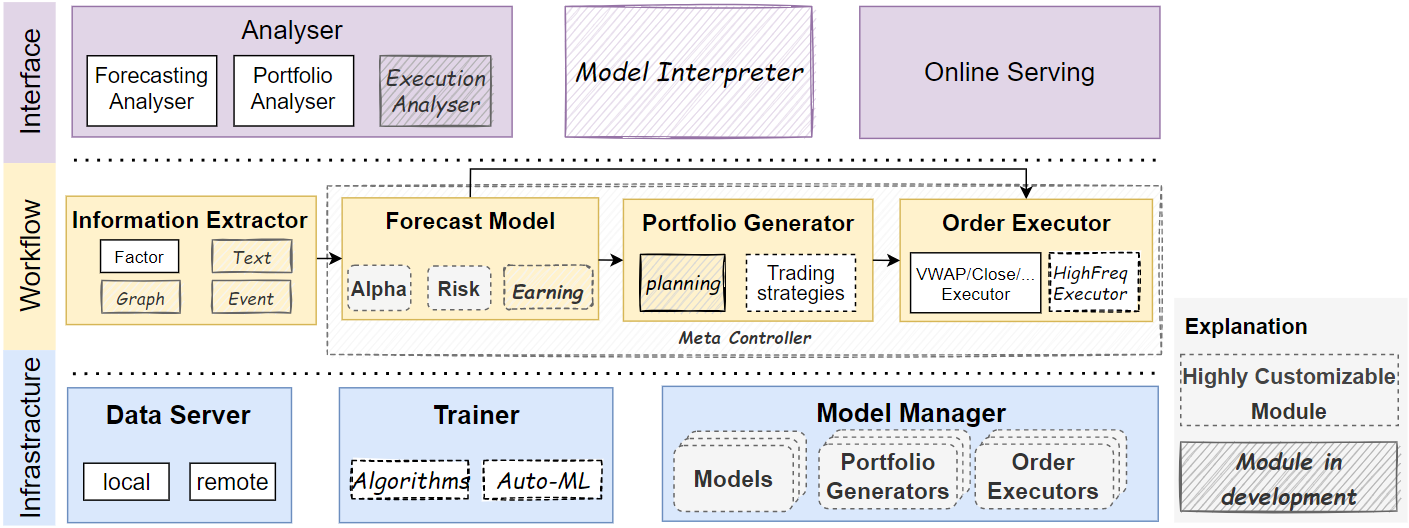
\includegraphics[width=0.5\textwidth]{framework.png}
    \caption{Quantitative Trading Framework Design.}
    \label{fig:framework}
\end{figure}

\subsection{\textbf{Data Feature Selection}}

The original price data consists of opening price, closing price, highest price, lowest price, trading volume, and restoration factor. With this information, various features can be created.

Heuristic principles for creating features include ensuring comparability across instruments by removing units from the features, thereby making them comparable between different instruments. Additionally, it is important to maintain distribution invariance, aiming to keep the distribution of features consistent to avoid biases. Finally, standardizing the feature scale is crucial to ensure that the scale of features is similar, which facilitates effective analysis and comparison.

The features encompass various aspects of market data, technical indicators, and statistical measures, enabling a holistic understanding of market dynamics. A total of 158 features have been created using ‘data loader’ provided by Qlib. These can be categorized into several key groups:

\begin{itemize}
    \item \textbf{Price and Volume Metrics:} Includes open, high, low, and volume-weighted average prices, as well as high and low prices over different time intervals.
    \item \textbf{Price Momentum and Rate of Change:} Rate of change metrics over different time periods, capturing momentum in price movements.
    \item \textbf{Moving Averages:} Moving averages over different time intervals to identify trends and potential reversal points.
    \item \textbf{Standard Deviation and Volatility:} Measures of volatility and dispersion, providing insights into market risk.
    \item \textbf{Beta and R-Squared:} Beta coefficients and R-squared values relative to benchmark indices, indicating asset volatility and correlation.
    \item \textbf{Regression Residuals and Statistical Measures:} Residuals from regression analysis and statistical measures to assess model fit and predictive power.
    \item \textbf{Min-Max Values and Quantiles:} Maximum and minimum values, as well as quantiles, offering insights into distribution and extremes.
    \item \textbf{Correlation and Counting Measures:} Correlation coefficients with other assets and counts of positive and negative changes.
    \item \textbf{Sum and Count Measures:} Sums of positive and negative changes over different time intervals, capturing cumulative market movements.
\end{itemize}

\subsection{\textbf{Selection of Quantitative Trading Models}}

In the prediction model section, the current choice is the LightGBM model, which is a gradient boosting framework based on decision trees. During the training process, LightGBM constructs a decision tree based on the target variable and input features, generating a stock ranking list that displays the importance score ranking of each stock.
After generating the ranking list, we can use a simple rule-based \texttt{TopkDropoutStrategy} to determine the target amount of each stock. The strategy adopts the Topk-Drop algorithm, which sells and buys a fixed number of stocks every trading day based on the prediction scores. The detailed steps of the \texttt{TopkDropoutStrategy} are as follows:

\begin{itemize}
    \item Adopt the Topk-Drop algorithm to calculate the target amount of each stock.
    
    There are two parameters for the Topk-Drop algorithm:
    \begin{itemize}
        \item \textbf{Topk}: The number of stocks held.
        \item \textbf{Drop}: The number of stocks sold on each trading day.
    \end{itemize}
    
    In general, the number of stocks currently held is \texttt{Topk}, with the exception of being zero at the beginning period of trading. For each trading day, let $d$ be the number of the instruments currently held and with a rank $K$ when ranked by the prediction scores from high to low. Then $d$ number of stocks currently held with the worst prediction score will be sold, and the same number of unheld stocks with the best prediction score will be bought.
    
    In general, $d=$ \texttt{Drop}, especially when the pool of the candidate instruments is large, $K$ is large, and \texttt{Drop} is small.
    
    In most cases, the Topk-Drop algorithm sells and buys \texttt{Drop} stocks every trading day, which yields a turnover rate of $2 \times \texttt{Drop} / K$.
    
    The following images illustrate a typical scenario.
    \begin{figure}[h]
        \centering
        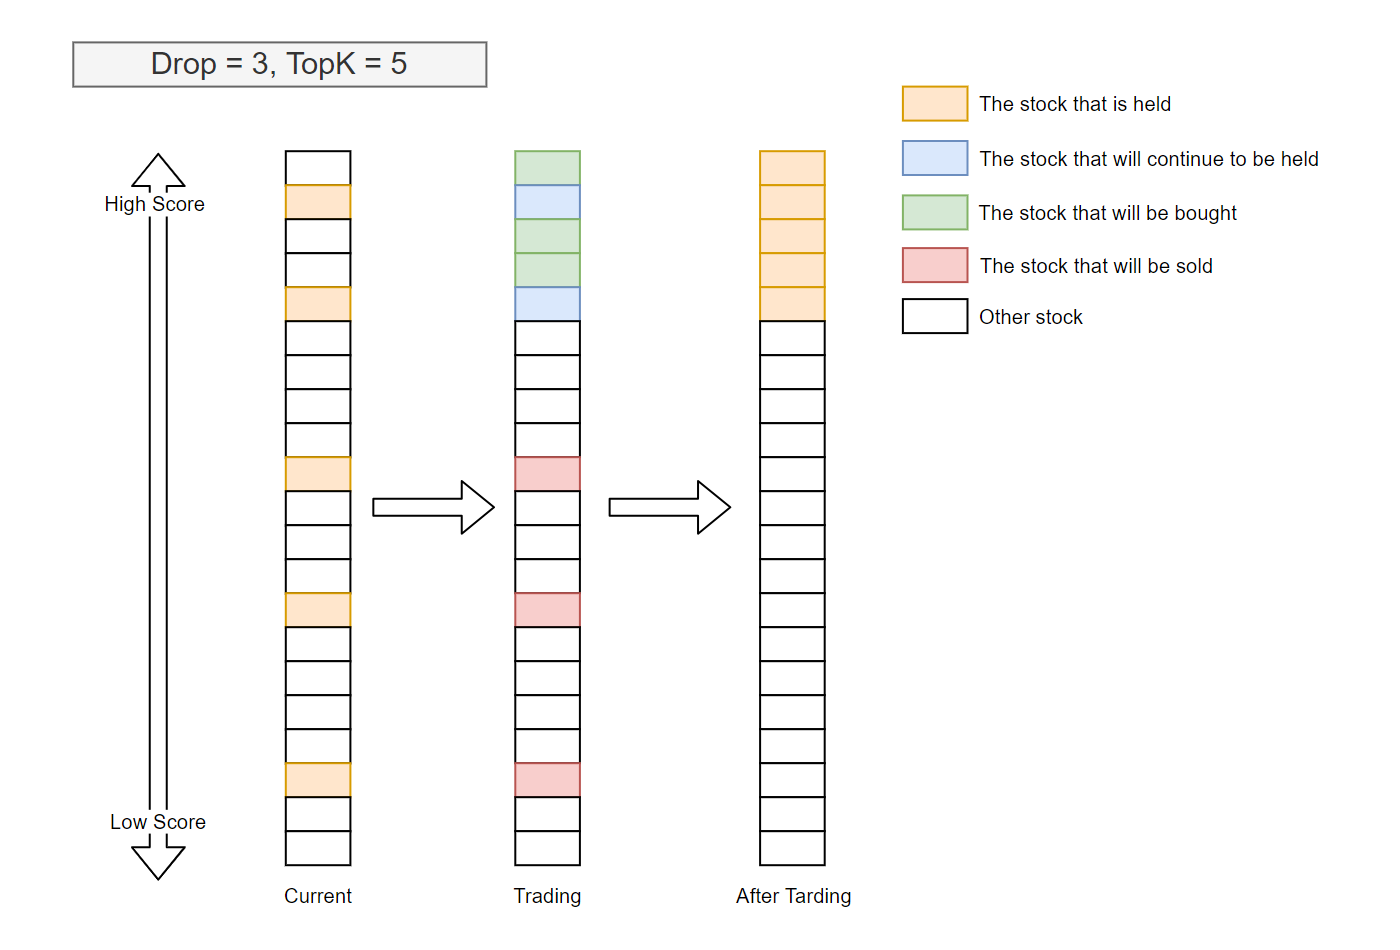
\includegraphics[width=0.5\textwidth]{topk_drop.png}
        \caption{TopkDropoutStrategy}
        \label{fig:TopkDropoutStrategy}
    \end{figure}
    \item Generate the order list from the target amount.
\end{itemize}

\section{\textbf{Backtesting Analysis}}
\subsection{\textbf{Market Sentiment Scores Produced by Fine-Tuned LLM}}

In practice, the datasets with social media and news reports in English for Twitter and other social media platforms are applied to fine-tune the language model. Specifically, given the text of news reports about market and company information, the language model is required to give the estimated sentiment value (i.e., -1, 0, or 1).

\begin{figure}[h]
    \centering
    \includegraphics[width=0.5\textwidth]{sentiment_score.png}
    \caption{Sentiment Scores Produced by Fine-tuned LLM.}
    \label{fig:sentiment scores}
\end{figure}

As illustrated in Figure \ref{fig:sentiment scores}, the fine-tuned language model can assign sentiment values based on the analysis of news articles. Compared to other existing sentiment estimation methods, large language models provide more precise sentiment perception results. Once the sentiment values are estimated, they are used to calculate sentiment factors. These sentiment factors are then combined with traditional financial factors, such as price-to-earnings ratios, market trends, and historical performance data, to create a hybrid factor set. This comprehensive feature set provides a richer and more nuanced input for subsequent prediction models used in trading strategies.

The sentiment estimation results can be further leveraged by exploiting the irrational behavior often observed in general market reactions. Since the language model is trained under human supervision and designed to mimic human behavior, its sentiment estimates reflect the general acknowledgment and mood of the market. By incorporating these sentiment insights, prediction models can identify and capitalize on market inefficiencies caused by irrational investor behavior.

For example, if the language model detects a predominantly negative sentiment towards a particular stock due to temporary negative news, but the fundamental financial indicators remain strong, the prediction model can anticipate a potential rebound once the market corrects its overreaction. Conversely, overly positive sentiment driven by hype can signal overvaluation, prompting a cautious investment approach.

\subsection{\textbf{Backtest Results of Quantitative Trading Strategies}}
\subsubsection*{\textbf{Backtesting Time}}
January 1, 2020 to August 1, 2022

\subsubsection*{\textbf{Benchmark}}
SPY, the SPDR S\&P 500 ETF trust, which is designed to track the S\&P 500 stock market index.

\subsubsection*{\textbf{Commission}}
0.0005

\begin{figure}[h!]
\centering
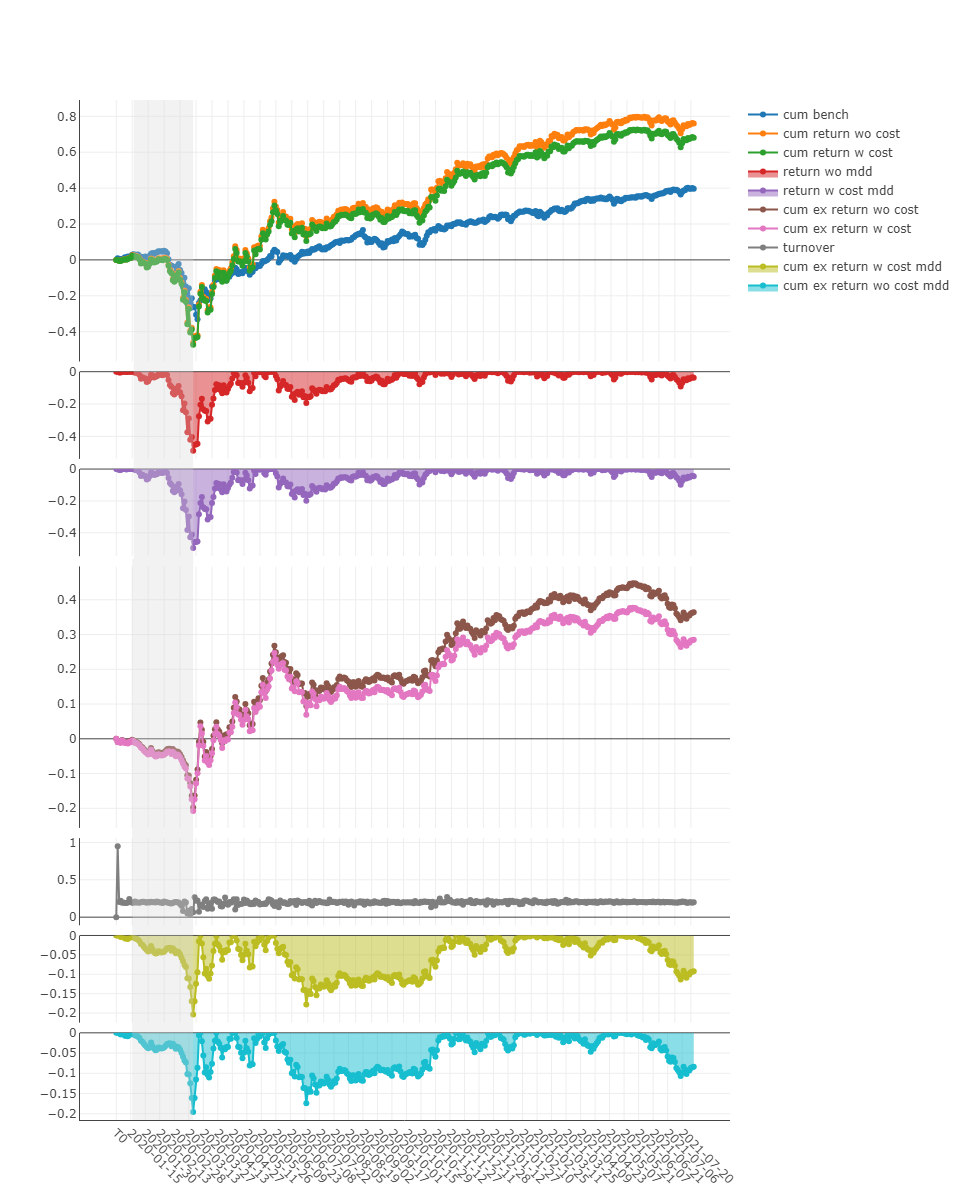
\includegraphics[width=0.5\textwidth]{plot_0.png}
\caption{Comprehensive Report}
\label{fig:comprehensive report}
\end{figure}

\subsection*{\textbf{Cumulative Returns (Cum Bench, Cum Return Wo Cost, Cum Return W Cost)}}

\textbf{Cum Bench:}
This line represents the cumulative returns of the benchmark, which is the SPY (SPDR S\&P 500 ETF Trust) in this case. The SPY tracks the S\&P 500 index, providing a benchmark for comparing the portfolio's performance.

\textbf{Cum Return Wo Cost:}
This line shows the cumulative returns of the portfolio without accounting for transaction costs.

\textbf{Cum Return W Cost:}
This line represents the cumulative returns of the portfolio after accounting for transaction costs (commission of 0.0005).

\subsection*{\textbf{Maximum Drawdown (Return Wo MDD, Return W Cost MDD)}}
\textbf{Return Wo MDD:}
Maximum drawdown series of the portfolio's cumulative return without transaction costs. Maximum drawdown measures the largest peak-to-trough decline in the portfolio's value.

\textbf{Return W Cost MDD:}
Similar to "Return Wo MDD" but includes the impact of transaction costs.

\subsection*{\textbf{Cumulative Abnormal Return (Cum Ex Return Wo Cost, Cum Ex Return W Cost)}}

\textbf{Cum Ex Return Wo Cost:}
The CAR (cumulative abnormal return) series of the portfolio compared to the benchmark, without considering transaction costs. It shows the excess return generated by the portfolio relative to the benchmark.

\textbf{Cum Ex Return W Cost:}
Similar to "Cum Ex Return Wo Cost" but includes transaction costs.

\subsection*{Turnover}
\textbf{Turnover:}
This line represents the portfolio's turnover rate, which is the frequency of buying and selling securities within the portfolio.

\subsection*{\textbf{Drawdown Series of CAR (Cum Ex Return W Cost MDD, Cum Ex Return Wo Cost MDD)}}
\textbf{Cum Ex Return W Cost MDD:}
Drawdown series of the CAR with transaction costs included.

\textbf{Cum Ex Return Wo Cost MDD:}
Similar to the above but without transaction costs.

\begin{center}
\subsection*{\textbf{Backtesting Performance Overview}}
\end{center}

Our quantitative model's backtesting performance from January 1, 2020, to August 1, 2022, as shown in the Figure~\ref{fig:comprehensive report}, indicates different performance characteristics. Here are possible reasons for performance variations:

\begin{enumerate}
    \item \textbf{Market Conditions}
    \begin{itemize}
        \item \textbf{January to April 2020:}
        \begin{itemize}
            \item \textbf{COVID-19 Pandemic:} The outbreak of COVID-19 led to extreme market volatility and a sharp decline in equity markets worldwide. Traditional models and strategies often struggle during periods of unprecedented events and high volatility. Even if our sentiment factor fine-tuned model still perform badly. This could explain the underperformance relative to SPY during this period.
            \item \textbf{Market Crash:} The market experienced a sudden crash in March 2020. Many quantitative models, especially those not specifically designed for extreme events, may have suffered during this time.
        \end{itemize}
        \item \textbf{May 2020 onwards:}
        \begin{itemize}
            \item \textbf{COVID-19 Pandemic:} From May 2020, markets began to recover as governments and central banks around the world implemented stimulus measures. This period saw a strong rebound in equity markets.
            \item \textbf{Market Crash:} Our model might be more effective during market recovery periods. If it is based on momentum, mean reversion, or other strategies that capitalize on trending markets, it would benefit from the sustained recovery and upward trend post-April 2020.
        \end{itemize}
    \end{itemize}

    \item \textbf{Strategy-Specific Factors}
    \begin{itemize}
        \item \textbf{January to April 2020:}
        \begin{itemize}
            \item \textbf{Strategy Limitations:} Our strategy relies on stable market conditions or specific economic indicators, it might have struggled during the early 2020 period of uncertainty and rapid changes.
            \item \textbf{Lagging Indicators:} Some strategies use indicators that lag behind actual market movements. During rapid declines, these models might not adjust quickly enough.
        \end{itemize}
        \item \textbf{May 2020 onwards:}
        \begin{itemize}
            \item \textbf{Effective Signal Processing:} Post-April 2020, as the market conditions stabilized and trends became more predictable, our model have been able to effectively process signals and generate excess returns.
            \item \textbf{Rebalancing and Optimization:} Since our model that include periodic rebalancing or dynamic optimization, it may cause perform better once the initial shock has passed and market signals are clearer.
        \end{itemize}
    \end{itemize}

    \item \textbf{Risk Management and Cost}
    \begin{itemize}
        \item \textbf{January to April 2020:}
        \begin{itemize}
            \item \textbf{High Volatility:} Increased volatility can lead to higher transaction costs and slippage, negatively impacting performance.
            \item \textbf{Risk Management Constraints:} Stringent risk management protocols might have resulted in more conservative positioning, leading to underperformance relative to a benchmark that does not adjust for risk as actively.
        \end{itemize}
        \item \textbf{May 2020 onwards:}
        \begin{itemize}
            \item \textbf{Improved Conditions:} As volatility decreased and markets trended upwards, the impact of transaction costs and slippage would be less severe.
            \item \textbf{Optimized Risk Management:} The model’s risk management strategies might have been more effective during stable market conditions, allowing for better performance relative to the benchmark.
        \end{itemize}
    \end{itemize}

\end{enumerate}

\begin{center}
    \subsection*{\textbf{Annualized Return}}
\end{center}

The annualized return measures the geometric average amount of money earned by an investment each year over a given time period, as shown in Figure~\ref{fig:annualized return}.

\begin{figure}[h!]
\centering
    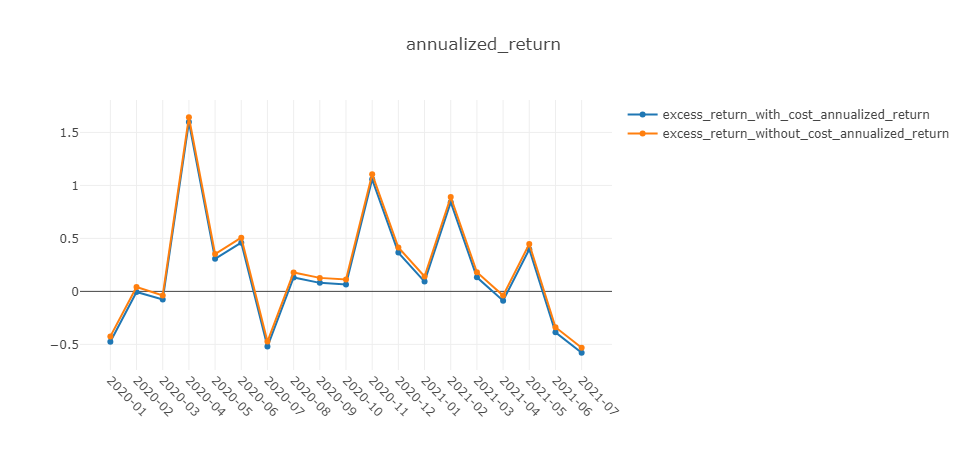
\includegraphics[width=0.5\textwidth]{annualized_return.png}
    \caption{Annualized Return}
    \label{fig:annualized return}
\end{figure}

\textbf{Analysis:}
\begin{itemize}
    \item \textbf{Volatility and Peaks:} The high volatility and peaks early in the chart (around April 2020) suggest that the model was capturing significant short-term gains. This might be attributed to the high market volatility due to the COVID-19 pandemic, where models that are responsive to rapid market movements can capture substantial returns.
    \item \textbf{Stabilization:} Post-2020, the annualized return stabilizes. This indicates that the model adapts well to varying market conditions, capturing consistent excess returns. The stability suggests effective signal processing and risk management mechanisms within the model.
    \item \textbf{Cost Impact:} The close alignment of returns with and without costs indicates low transaction costs, which is beneficial for high-frequency trading models.
\end{itemize}

\begin{center}
    \subsection*{\textbf{Maximum Drawdown}}
\end{center}

Maximum drawdown represents the largest drop from a peak to a trough before a new peak is attained. It is a critical measure of downside risk, as shown in Figure~\ref{fig:maximum drawdown}.

\begin{figure}[h!]
\centering
    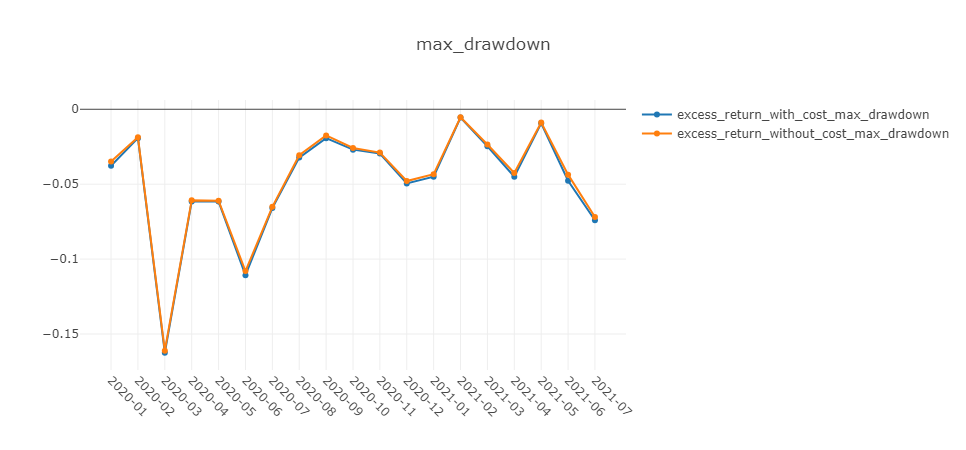
\includegraphics[width=0.5\textwidth]{max_drawdown.png}
    \caption{Maximum Drawdown}
    \label{fig:maximum drawdown}
\end{figure}

\textbf{Analysis:}
\begin{itemize}
    \item \textbf{Initial Drawdown:} The sharp drawdown in early 2020 corresponds with the market crash due to the pandemic. This significant drawdown highlights the model's initial struggle during extreme market conditions.
    \item \textbf{Risk Management:} The reduced drawdowns post-2020 indicate improved risk management. The model's ability to minimize losses after the initial market shock suggests effective adaptation to market recovery.
    \item \textbf{Drawdown Consistency:} The similar patterns of drawdowns with and without costs show that the cost factor has a minimal impact on risk during this period, which is a positive sign for the strategy's robustness and prove that our workflow is cost-efficient in high-frequency trading.
\end{itemize}

\begin{center}
    \subsection*{\textbf{Information Ratio}}
\end{center}

The information ratio is a measure of portfolio returns beyond the returns of a benchmark, usually an index, here we use SP500 as the benchmark, as shown in Figure~\ref{fig:information ratio}.

\begin{figure}[h!]
\centering
    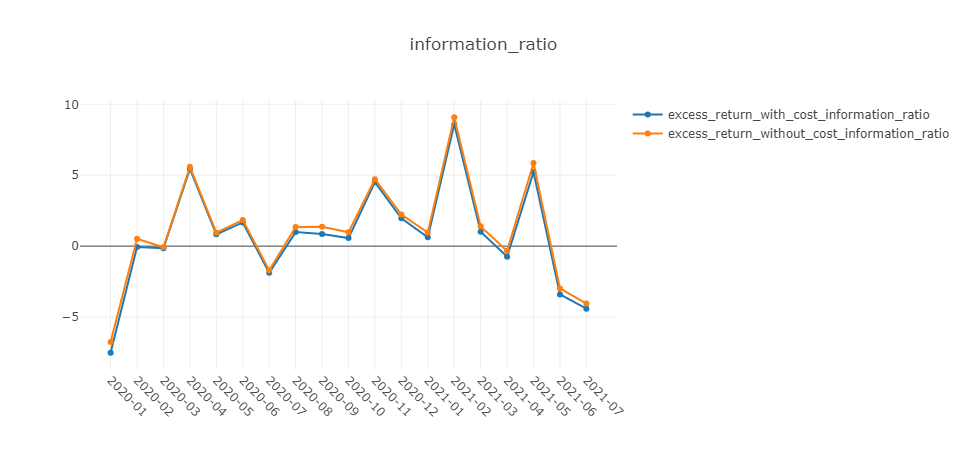
\includegraphics[width=0.5\textwidth]{information_ratio.png}
    \caption{Information Ratio}
    \label{fig:information ratio}
\end{figure}

\textbf{Analysis:}
\begin{itemize}
    \item \textbf{Performance Peaks:} Peaks in the information ratio indicate periods where the model generated high risk-adjusted returns, notably around April 2020 and early 2021. This shows the model's effectiveness in generating excess returns relative to the risk taken during these periods.
    \item \textbf{Consistent Performance:} The consistent positive information ratio over time reflects the model's ability to continuously generate alpha. This is crucial for strategies aimed at outperforming benchmarks consistently. At the most time, the information ratio is above 0, which means our model is outperforming the benchmark.
    \item \textbf{Cost Impact:} The close tracking of the information ratio with and without costs suggests that the strategy is cost-efficient, maintaining high risk-adjusted returns even after accounting for transaction costs.
\end{itemize}

\begin{center}
    \subsection*{\textbf{Standard Deviation}}
\end{center}

Standard deviation measures the amount of variability or dispersion around the mean return of an investment, as shown in Figure~\ref{fig:standard deviation}.

\begin{figure}[h!]
\centering
    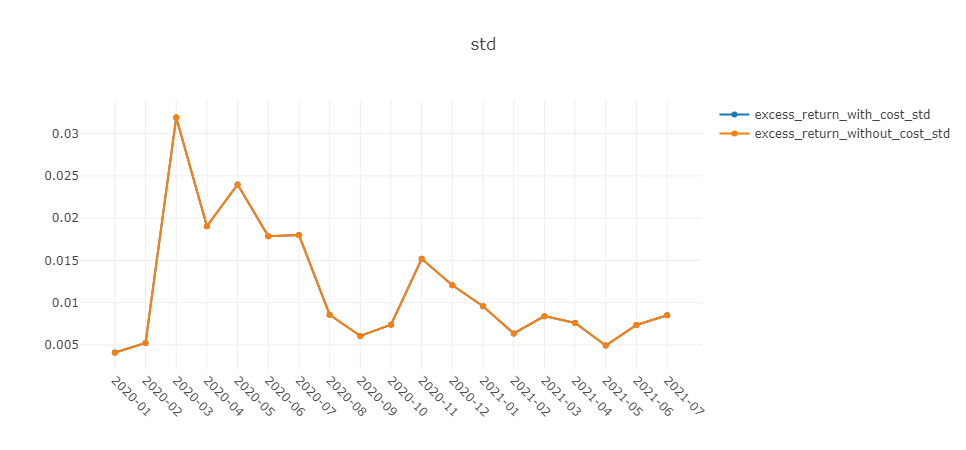
\includegraphics[width=0.5\textwidth]{std.png}
    \caption{Standard Deviation}
    \label{fig:standard deviation}
\end{figure}

\textbf{Analysis:}
\begin{itemize}
    \item \textbf{High Initial Volatility:} Early 2020 shows high standard deviation, indicating significant volatility due to the market turmoil caused by the pandemic.
    \item \textbf{Decreasing Volatility:} The reduction in standard deviation over time signifies a stabilization of the model's returns. Lower volatility post-2020 suggests that the market conditions became more predictable and the model adapted to these conditions.
    \item \textbf{Model Stability:} The declining standard deviation implies that the model's risk (in terms of return variability) has decreased, which is a positive sign of its robustness and reliability over time.
\end{itemize}

\section{\textbf{Strategy Summary}}

\subsection{\textbf{Problem Analysis}}

The backtesting performance of our quantitative model from January 1, 2020, to August 1, 2022, highlighted several key areas of concern and areas for improvement:

\begin{itemize}
    \item \textbf{Initial Underperformance}: From January to April 2020, the model underperformed relative to the benchmark (SPY). This period coincided with the onset of the COVID-19 pandemic, which caused extreme market volatility and sharp declines. The model struggled to adapt to these unprecedented conditions, resulting in significant drawdowns and underperformance.
    \item \textbf{Volatility Sensitivity}: The model exhibited high sensitivity to market volatility. During periods of high volatility, such as the market crash in March 2020, the model's performance deteriorated, leading to significant drawdowns. This indicates that the model's risk management and volatility adjustment mechanisms were insufficient during extreme market conditions.
    \item \textbf{Single Model Limitation}: The current strategy relies solely on a decision-tree-based model, specifically LightGBM. While LightGBM is powerful, it may not be the optimal choice for all market conditions, especially when dealing with a diverse set of factors such as price-volume combinations and sentiment factors.
\end{itemize}

\subsection{\textbf{Proposed Improvements}}

To address the identified issues and enhance the model's performance, several improvements are proposed:

\begin{itemize}
    \item \textbf{Diversify Prediction Models}: Relying on a single model (LightGBM) limits the strategy's adaptability and robustness. To improve performance, we should experiment with and incorporate multiple models, including but not limited to:
    \begin{itemize}
        \item \textbf{Random Forests}: For their robustness and ability to handle noisy data.
        \item \textbf{Gradient Boosting Machines}: Besides LightGBM, explore alternatives like XGBoost and CatBoost.
        \item \textbf{Neural Networks}: Especially deep learning models that can capture complex patterns and interactions in the data.
        \item \textbf{Support Vector Machines (SVM)}: For their effectiveness in high-dimensional spaces.
    \end{itemize}
    \item \textbf{Enhanced Volatility Management}: Implement advanced volatility-adjusted strategies to better manage risk during periods of high market volatility. Techniques such as dynamic volatility scaling, regime-switching models, or incorporating volatility indices (e.g., VIX) can help the model adapt to changing market conditions.
    \item \textbf{Sentiment Analysis Integration}: While our current model incorporates sentiment factors, there is room for improvement in how these factors are integrated. Advanced natural language processing (NLP) techniques, such as transformers (e.g., BERT, GPT-3), can be utilized to extract more nuanced sentiment signals from textual data, potentially improving the model's predictive power.
    \item \textbf{Regular Model Evaluation and Tuning}: Establish a robust framework for continuous model evaluation and hyperparameter tuning. This includes implementing automated machine learning (AutoML) techniques to regularly assess and optimize model parameters, ensuring the strategy remains aligned with current market dynamics.
    \item \textbf{Feature Engineering and Selection}: Enhance the feature engineering process to identify and incorporate additional predictive factors. Techniques such as feature importance analysis, principal component analysis (PCA), and clustering can help identify and select the most relevant features, improving model accuracy and robustness.
\end{itemize}

\subsection{\textbf{Additional Recommendations}}

\begin{itemize}
    \item \textbf{Incorporate Twitter Sentiment Analysis}: Beyond analyzing news sentiment, incorporating sentiment analysis of social media platforms like Twitter could provide valuable insights. Since individual investors' sentiments on platforms like Twitter may often be reactionary and less informed, they could serve as contrarian indicators. Conversely, authoritative news sources can be used as positive indicators due to their more reliable and analyzed content.
    \item \textbf{Utilize Specialized Sentiment Models}: While large models like Llama 3 have strong generalization capabilities, they might not always outperform specialized models in niche domains. Using smaller, domain-specific sentiment analysis models fine-tuned for financial texts may yield better results in extracting relevant sentiment signals from financial news and social media content.
\end{itemize}

\begin{thebibliography}{00}
\bibitem{b1} X. Yang, W. Liu, D. Zhou, J. Bian, and T.-Y. Liu, “Qlib: An AI-oriented Quantitative Investment Platform.” arXiv, Sep. 22, 2020. Accessed: Jun. 21, 2024. [Online]. Available: http://arxiv.org/abs/2009.11189
\end{thebibliography}

\end{document}
